\chapter{Marco Teórico}
\label{cp:marco-teorico}

Este capítulo establece las bases teóricas y conceptuales que fundamentan el desarrollo del proyecto TechSolutions Pro. Se abordan los componentes principales que sustentan la metodología y las tecnologías empleadas: la metodología Jesse James Garrett para User Experience Design y el framework Angular 19 con sus tecnologías asociadas.

\section{Metodología Jesse James Garrett}

\subsection{Contexto Histórico y Fundamentos}

Jesse James Garrett, reconocido diseñador y consultor en experiencia de usuario, estableció en el año 2000 una metodología revolucionaria a través de su obra seminal ``The Elements of User Experience: User-Centered Design for the Web''. Esta metodología surge como respuesta a la necesidad de estructurar y sistematizar el proceso de diseño centrado en el usuario en el desarrollo web, proporcionando un marco conceptual que ha influenciado profundamente la industria del diseño digital durante más de dos décadas.

La metodología de Garrett se fundamenta en la premisa de que la experiencia del usuario no es un elemento aislado, sino el resultado de decisiones interdependientes que se toman en diferentes niveles de abstracción durante el proceso de desarrollo. Su enfoque holístico considera tanto los aspectos funcionales como los estéticos, integrándolos en un modelo coherente y aplicable.

\subsection{Las Cinco Capas de la Metodología}

La metodología Jesse James Garrett se estructura en cinco capas distintas pero interconectadas, cada una con objetivos específicos y entregables concretos. Estas capas se construyen de manera secuencial, desde los niveles más abstractos hasta los más concretos.

\begin{figure}[htbp]
    \centering
    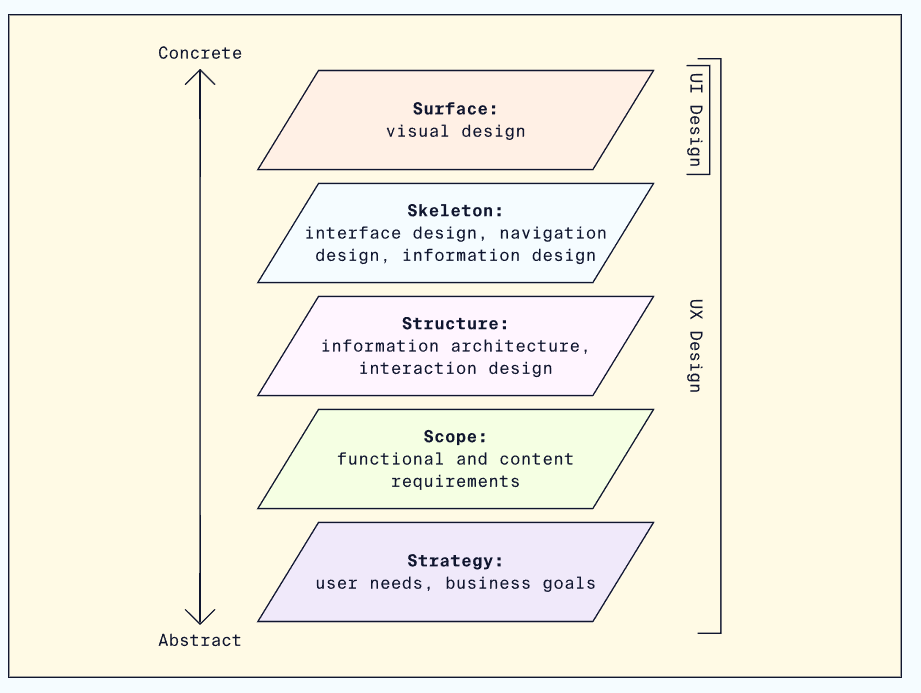
\includegraphics[width=0.8\textwidth]{Figures/ux.png}
    \caption{Modelo de las Cinco Capas de la Metodología Jesse James Garrett}
    \label{fig:ux-methodology}
\end{figure}

Como se observa en la Figura \ref{fig:ux-methodology}, el modelo se presenta como una serie de planos superpuestos que van desde lo abstracto (Strategy) hasta lo concreto (Surface), donde cada capa se apoya en las decisiones tomadas en las capas inferiores. El lado izquierdo representa el área de diseño funcional, mientras que el lado derecho corresponde al diseño de información, convergiendo ambos en la capa superior de superficie visual.

\subsubsection{Capa 1: Strategy (Estrategia)}

La capa de estrategia constituye el fundamento conceptual de todo el proyecto. En esta fase se definen los objetivos de negocio y se identifican las necesidades específicas de los usuarios. Los elementos principales incluyen:

\begin{itemize}
    \item \textbf{Objetivos de negocio}: Definición clara de los propósitos corporativos que el sitio web debe cumplir
    \item \textbf{Necesidades del usuario}: Identificación y análisis de las expectativas, motivaciones y limitaciones de la audiencia objetivo
    \item \textbf{Análisis competitivo}: Evaluación del contexto competitivo y identificación de oportunidades de diferenciación
    \item \textbf{Propuesta de valor}: Articulación del valor único que el sitio web proporcionará a sus usuarios
\end{itemize}

\subsubsection{Capa 2: Scope (Alcance)}

La capa de alcance traduce las decisiones estratégicas en especificaciones concretas sobre lo que el sitio web debe hacer y contener. Esta fase comprende:

\begin{itemize}
    \item \textbf{Especificaciones funcionales}: Definición detallada de las características y comportamientos del sitio
    \item \textbf{Requerimientos de contenido}: Identificación del tipo, volumen y estructura del contenido necesario
    \item \textbf{Priorización de características}: Clasificación de funcionalidades según su importancia estratégica
    \item \textbf{Constraints y limitaciones}: Reconocimiento de las restricciones técnicas, temporales y presupuestarias
\end{itemize}

\subsubsection{Capa 3: Structure (Estructura)}

La capa de estructura se enfoca en la organización y interacción de los elementos definidos en el alcance. Sus componentes principales son:

\begin{itemize}
    \item \textbf{Arquitectura de información}: Organización, etiquetado y estructuración del contenido
    \item \textbf{Diseño de interacción}: Definición de cómo los usuarios interactuarán con las funcionalidades
    \item \textbf{Flujos de usuario}: Mapeo de los caminos que los usuarios seguirán para completar tareas
    \item \textbf{Taxonomías y categorización}: Sistemas de clasificación que faciliten la navegación y búsqueda
\end{itemize}

\subsubsection{Capa 4: Skeleton (Esqueleto)}

La capa de esqueleto establece la disposición y priorización de los elementos de interfaz. Esta fase incluye:

\begin{itemize}
    \item \textbf{Diseño de interfaz}: Ubicación y jerarquía de elementos en cada página
    \item \textbf{Diseño de navegación}: Sistemas de navegación que soporten los flujos de usuario
    \item \textbf{Diseño de información}: Presentación y priorización del contenido
    \item \textbf{Wireframing}: Representaciones esquemáticas de la estructura de las páginas
\end{itemize}

\subsubsection{Capa 5: Surface (Superficie)}

La capa de superficie se centra en los aspectos sensoriales y estéticos de la experiencia del usuario:

\begin{itemize}
    \item \textbf{Diseño visual}: Selección de colores, tipografías, imágenes y elementos gráficos
    \item \textbf{Diseño sensorial}: Consideración de aspectos auditivos, táctiles y de movimiento
    \item \textbf{Identidad de marca}: Aplicación coherente de los elementos de identidad corporativa
    \item \textbf{Accesibilidad visual}: Garantía de que el diseño sea accesible para usuarios con diversas capacidades
\end{itemize}

\subsection{Ventajas y Beneficios de la Metodología}

La aplicación de la metodología Jesse James Garrett proporciona múltiples beneficios para el desarrollo de proyectos web:

\begin{itemize}
    \item \textbf{Estructura sistemática}: Proporciona un marco organizativo claro que reduce la ambigüedad
    \item \textbf{Reducción de riesgos}: Identifica problemas potenciales en fases tempranas del desarrollo
    \item \textbf{Enfoque centrado en el usuario}: Garantiza que las decisiones de diseño se basen en necesidades reales
    \item \textbf{Comunicación efectiva}: Facilita la comunicación entre equipos multidisciplinarios
    \item \textbf{Escalabilidad}: Permite aplicar el método en proyectos de diversa complejidad
\end{itemize}

\subsection{Aplicación en Desarrollo Web Moderno}

La metodología de Garrett ha demostrado su relevancia y adaptabilidad en el contexto del desarrollo web moderno. Su aplicación en frameworks como Angular permite:

\begin{itemize}
    \item Integración natural con metodologías ágiles de desarrollo
    \item Aplicación de principios UX en arquitecturas de componentes
    \item Validación continua de decisiones de diseño durante el desarrollo
    \item Optimización de la experiencia del usuario en aplicaciones de página única (SPA)
\end{itemize}

\section{Angular 19 y Tecnologías Asociadas}

\subsection{Angular 19: Framework para Aplicaciones Web Modernas}

Angular 19 representa la evolución más reciente del framework desarrollado por Google para la creación de aplicaciones web robustas y escalables. Esta versión introduce innovaciones significativas que mejoran tanto la experiencia del desarrollador como el rendimiento de las aplicaciones resultantes.

\subsubsection{Características Principales de Angular 19}

\begin{itemize}
    \item \textbf{Componentes Standalone}: Eliminación de la dependencia obligatoria de NgModules, simplificando la arquitectura
    \item \textbf{Sistema de Signals}: Nuevo sistema de reactividad que mejora la detección de cambios
    \item \textbf{Lazy Loading optimizado}: Mejoras en la carga diferida de componentes y módulos
    \item \textbf{Bundle size reducido}: Optimizaciones que resultan en aplicaciones más ligeras
    \item \textbf{Mejor rendimiento}: Optimizaciones en el ciclo de vida de componentes y detección de cambios
\end{itemize}

\subsubsection{Componentes Standalone}

Los componentes standalone representan un cambio paradigmático en la arquitectura de Angular, permitiendo:

\begin{itemize}
    \item Creación de componentes sin dependencia de NgModules
    \item Imports directos de dependencias en el componente
    \item Simplificación de la estructura de proyectos
    \item Mejor tree-shaking y optimización de bundles
    \item Facilitar la migración y modularización
\end{itemize}

\subsection{TypeScript: Lenguaje de Programación}

TypeScript constituye la base del desarrollo en Angular, proporcionando tipado estático sobre JavaScript. Sus características principales incluyen:

\begin{itemize}
    \item \textbf{Tipado estático}: Detección de errores en tiempo de compilación
    \item \textbf{Programación orientada a objetos}: Soporte completo para clases, interfaces y herencia
    \item \textbf{Interfaces}: Definición de contratos para objetos y funciones
    \item \textbf{Decoradores}: Metaprogramación para extender funcionalidad de clases y métodos
    \item \textbf{Compatibilidad con ES6+}: Soporte para características modernas de JavaScript
\end{itemize}

\subsection{SCSS: Preprocesador de CSS}

SCSS (Sassy CSS) extiende las capacidades de CSS estándar, ofreciendo:

\begin{itemize}
    \item \textbf{Variables}: Reutilización de valores a lo largo de los estilos
    \item \textbf{Mixins}: Grupos reutilizables de declaraciones CSS
    \item \textbf{Anidación}: Organización jerárquica de selectores
    \item \textbf{Partials e imports}: Modularización de archivos de estilos
    \item \textbf{Funciones}: Lógica programática en la generación de estilos
\end{itemize}

\subsection{Reactive Forms: Gestión de Formularios}

El sistema de Reactive Forms de Angular proporciona:

\begin{itemize}
    \item \textbf{Validación robusta}: Sistema extensible de validadores síncronos y asíncronos
    \item \textbf{Control de estados}: Gestión detallada de estados de campos y formularios
    \item \textbf{Programación reactiva}: Integración con observables para manejo de eventos
    \item \textbf{Validación cruzada}: Validadores que consideran múltiples campos
    \item \textbf{Mensajes de error dinámicos}: Sistema flexible para mostrar errores contextuales
\end{itemize}

\subsection{Angular Router: Navegación y Enrutamiento}

El sistema de routing de Angular 19 incluye capacidades avanzadas:

\begin{itemize}
    \item \textbf{Lazy loading}: Carga diferida de componentes y módulos
    \item \textbf{Guards}: Protección de rutas con lógica de autorización
    \item \textbf{Resolvers}: Pre-carga de datos antes de navegar a una ruta
    \item \textbf{Parámetros dinámicos}: Rutas parametrizadas para contenido dinámico
    \item \textbf{Navegación programática}: Control de navegación desde componentes
\end{itemize}

\subsection{RxJS: Programación Reactiva}

RxJS (Reactive Extensions for JavaScript) proporciona herramientas para programación reactiva:

\begin{itemize}
    \item \textbf{Observables}: Streams de datos asíncronos
    \item \textbf{Operadores}: Transformación y manipulación de streams
    \item \textbf{Gestión de estado}: Patrones para manejo de estado aplicacional
    \item \textbf{Manejo de errores}: Estrategias robustas para gestión de errores asíncronos
    \item \textbf{Composición}: Combinación de múltiples fuentes de datos
\end{itemize}

\section{Integración de Metodología UX y Tecnología}

La convergencia entre la metodología Jesse James Garrett y Angular 19 representa una oportunidad única para crear experiencias digitales excepcionales. Esta integración permite:

\begin{itemize}
    \item Aplicar principios UX estructurados en arquitecturas de componentes modernas
    \item Validar decisiones de diseño mediante prototipado rápido
    \item Implementar diseños responsive que se adapten a múltiples dispositivos
    \item Crear interfaces interactivas que respondan eficientemente a las acciones del usuario
    \item Optimizar el rendimiento sin comprometer la experiencia del usuario
\end{itemize}

La metodología de Garrett proporciona el marco conceptual para tomar decisiones de diseño fundamentadas, mientras que Angular 19 ofrece las herramientas técnicas para implementar estas decisiones de manera eficiente y mantenible. Esta combinación resulta en aplicaciones web que no solo cumplen con los objetivos de negocio, sino que también proporcionan experiencias de usuario excepcionales y código de alta calidad.
